
\subsection{Metody kodowania}
\subsubsection{Notacja Gaußa}
\index{notacja!Gaußa|(}%
Pierwszymi osobami, które zajmowały się węzłami, był prawdopodobnie Gauß oraz jego uczeń, Listing.
\index[persons]{Gauß, Carl}%
\index[persons]{Listing, Johann}%
Gauß wprowadził indeks zaczepienia dwóch węzłów jako pewna całka oraz notację dla węzłów.
Wybierzmy punkt na diagramie, który nie jest skrzyżowaniem i przemierzajmy go zgodnie z~orientacją.
Gdy mijamy nowe skrzyżowania, przypisujemy im kolejne liczby $1, 2, \ldots$, zaś dla starych skrzyżowań przepisujemy numer.
Jeżeli mijamy skrzyżowanie dołem, kodujemy je liczbą z minusem.

\begin{comment}
\begin{figure}[H]
    \centering
    \begin{minipage}[b]{.45\linewidth}
        \centering
        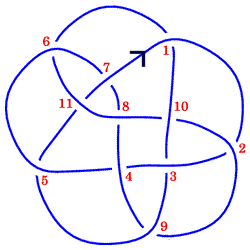
\includegraphics[width=0.90\linewidth]{../data/mixed/gauss_code.png}
        \subcaption{Węzeł o kodzie Gaußa 1 -2 3 -4 5 6 -7 -8 4 -9 2 -10 8 11 -6 -1 10 -3 9 -5 -11 7. Źródło:\\ \url{https://knotinfo.math.indiana.edu/descriptions/gauss_notation.html}.}
    \end{minipage}
    \quad
    \begin{minipage}[b]{.45\linewidth}
        \centering
        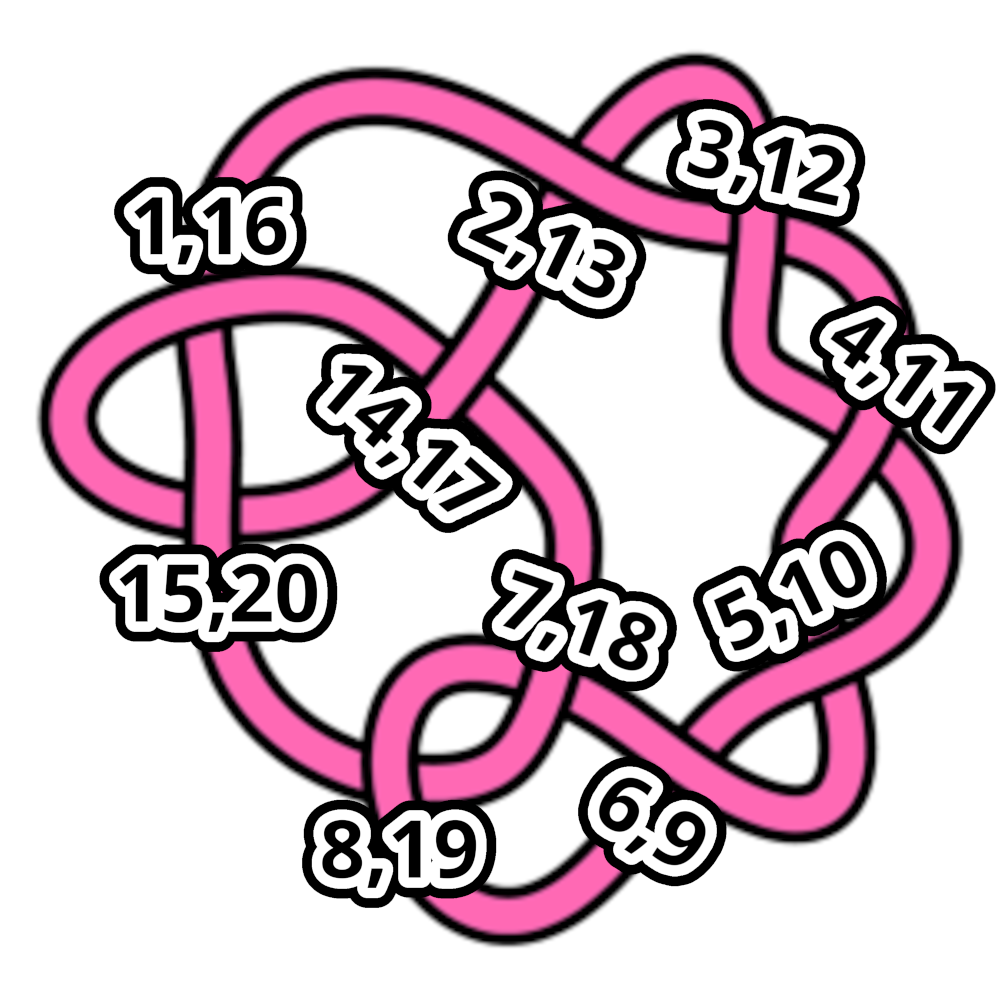
\includegraphics[width=0.90\linewidth]{../data/mixed/dowker_code.png}
        \subcaption{o kodzie (Dowkera-Thistlethwaite'a) 16 18 20 -22 4 2 8 -6 12 10 -14. Źródło:\\ \url{https://knotinfo.math.indiana.edu/descriptions/dt_notation.html}.}
    \end{minipage}
\end{figure}
\end{comment}

W ogólnym przypadku nie można odtworzyć węzła z jego kodu, ale można delikatnie zmienić notację, by było to możliwe.
Kiedy mijamy skrzyżowanie drugi raz, stawiamy minus przed liczbą, jeżeli skrzyżowanie jest lewoskrętne i plus w przeciwnym wypadku.
Nazywa się to rozszerzonym kodem Gaußa.
W naszym przykładzie, rozszerzony kod to 1 -2 3 -4 5 6 -7 -8 \textbf{-4} -9 \textbf{-2} -10 8 11 \textbf{6 -1 -10 3 9 -5 -11 -7}, pogrubione liczby odpowiadają drugim przejściom.

\index{notacja!Gaußa|)}%

\subsubsection{Notacja Dowkera-Thistlethwaite'a}
\index{notacja!Taita}
\index{notacja!Dowkera-Thistlethwaite'a|(}
Poprawia nieopisaną tutaj notację Taita, opisana po raz pierwszy w~pracy \cite{dowker83}.
\index[persons]{Dowker, Clifford}%
\index[persons]{Thistlethwaite, Morwen}%

Tak jak w~notacji Gaußa, przemierzamy węzeł zaczynając poza skrzyżowaniem.
Tym razem jednak stare skrzyżowania dostają drugi, nowy numer.
Jak można zauważyć, każde skrzyżowanie ma parzystą oraz nieparzystą etykietę.

\begin{definition}
    Ciąg parzystych liczb występujących na diagramie kolejno przy $1, 3, \ldots$ nazywamy kodem Dowkera-Thistlethwaite'a.
    Jeżeli nieparzysta etykieta odpowiadała podskrzyżowaniu, zapisujemy liczbę z~minusem.
\end{definition}

Opisany powyżej kod nie jest idealny, ponieważ odtworzony z niego węzeł może być lustrzanym odbiciem wyjściowego.
Ogólniej, odbicie dowolnego składnika sumy spójnej nie zmienia kodu całego węzła.
Nie stanowi to jednak dużego problemu, ponieważ notacja została stworzona na potrzeby tablicowania węzłów pierwszych, a~te są niezorientowane.

Zaczynając od zredukowanego diagramu o $n$ skrzyżowaniach nie można doprowadzić do sytuacji, gdzie do pewnego skrzyżowania przypisane są dwie kolejne liczby całkowite.
Dzięki temu problem można przetłumaczyć na język teorii grafów.
Rozpatrzmy graf $G$, którego wierzchołkami są liczby $1, 2, \ldots, 2n$.
Połączmy niesąsiadujące modulo $2n$ wierzchołki o różnej parzystości krawędziami.
Graf ten powstaje przez usunięcie cyklu Hamiltona (łączącego kolejne liczby) z pełnego grafu dwudzielnego.
Zbiór par etykiet przy skrzyżowaniach węzła to skojarzenie doskonałe w grafie $G$.
Liczba skojarzeń prawie pokrywa się z rozwiązaniem zadania znanego w literaturze jako ,,problème des ménages'': na ile sposobów $n$ małżeństw można posadzić przy okrągłym stole tak, by żadne małżeństwo nie siedziało obok siebie i~każdy mężczyzna znalazł się obok dwóch kobiet?
Ustawienia, które powstają przez cykliczne permutowanie należy uznać za tożsame.
Gilbert znalazł w \cite{gilbert56} wzór na $a_n$, liczbę różnych kodów:
\begin{align}
u(m, t) & = 2m \sum_{k=0}^m {2m-k \choose k} \cdot (m-k)! \cdot \frac{(t-1)^k}{2m - k}  \\
a(n) & = \frac{1}{n} \sum_{d\mid n} \left(\frac{n}{d}\right)^d \cdot u \left(d, 1 - \frac{d}{n}\right) \cdot \varphi \left(\frac{n}{d}\right)
\end{align}

Kilka początkowych wartości to $a_3 = 1, 2, 5, 20, 87, 616, 4843, 44128, 444621, \ldots$ (ciąg A002484 w OEIS).

\index{notacja!Dowkera-Thistlethwaite'a|)}%

\subsubsection{Notacja Alexandera-Briggsa}
\index{notacja!Alexandera-Briggsa|(}%
W~1927 roku Alexander, Briggs wprowadzili zupełnie inny sposób oznaczania węzłów -- wtedy do 9 skrzyżowań, ale przedłużoną do 10 skrzyżowań przez Rolfsena i używaną po dziś dzień.
Do opisu węzła używa się dwóch liczb: jego indeksu skrzyżowaniowanego z dolnym indeksem, oznaczającym miejsce w tablicy~węzłów.
I~tak węzły o~ośmiu skrzyżowaniach to $8_1, 8_2, \ldots,$ $8_{21}$.
Porządek jest umowny i jego wybór należy do osoby, która jako pierwsza znajdzie wszystkie węzły o danej liczbie skrzyżowań (ale węzeł skręcony występuje zawsze po torusowym).
\index{węzeł!skręcony}%
\index{węzeł!torusowy}%

Od jedenastu skrzyżowań pojawia się mała zmiana: węzły alternujące i niealternujące kataloguje się osobno.
I tak $11n_{185}$ to sto osiemdziesiąty piąty węzeł niealternujący o 11 skrzyżowaniach, zaś $11a_{367}$ to trzysta sześćdziesiąty siódmy alternujący.

Rolfsen w 1976 stworzył z kilkoma błędami tablicę diagramów pierwszych węzłów do 10 skrzyżowań.
Para Perko $10_{161}, 10_{162}$ przedstawia ten sam węzeł, zaś górne skrzyżowanie w~$10_{144}$ powinno być zmienione.
Ostatnie cztery węzły dostały nowe numery, by uniknąć duplikatu.
Kolejną usterką tablicy jest to, że notacja Conwaya oraz wielomian Alexandera dla węzłów $10_{83}$ oraz $10_{86}$ są zamienione miejscami.
Tu czyha pułapka:\footnote{Wiemy o niej dzięki stronie \url{http://stoimenov.net/stoimeno/homepage/ptab/}.} Stojmenow, nowe wydanie książki Rolfsena, atlas węzłów Bar-Natana oraz tablica niezmienników węzłowych Livingstona naprawiają to przez wymianę podpisów.
Podręcznik Kawauchiego wymienia diagramy.

Ze strony internetowej Stojmenowa dowiedzieliśmy się jeszcze czegoś.
Kolejność Rolfsena dla węzłów o 10 skrzyżowaniach obala nomenklaturę Little'a niealternujących oraz nadpisuje numerowanie Taita dla alternujących węzłów.
Alexander, Briggs zrobili wcześniej to samo dla 9 lub mniej skrzyżowań.

\index{notacja!Alexandera-Briggsa|)}%

\subsubsection{Notacja Conwaya}
\index{notacja!Conwaya}%
Wprowadzona przez Conwaya w~pracy \cite{conway70}.
Wymaga znajomości supłów, więc przedstawiamy ją w sekcji supłów: definicji \ref{conway_notation}.

\subsubsection{Nazwy zwyczajowe}
Niektóre węzły i sploty, w szczególności te o niskim indeksie skrzyżowaniowym, występują tak często w teorii węzłów, że doczekały się nazw zwyczajowych.
Oto ich lista:
\begin{compactitem}
% DICTIONARY;unknot;niewęzeł;-
% TODO: nigdzie w książce nie ma definicji niesplotu?
    \item węzeł $0_1$ to niewęzeł;
% DICTIONARY;trefoil knot;trójlistnik;-
    \item węzeł $3_1$ to trójlistnik,
% DICTIONARY;figure-eight;ósemka;-
    \item węzeł $4_1$ to ósemka albo węzeł Listinga,
% DICTIONARY;cinquefoil knot;pięciolistnik;-
    \item węzeł $5_1$ to pięciolistnik albo węzeł Solomona (!),
% DICTIONARY;stevedore knot;węzeł dokerski;-
    \item węzeł $6_1$ to węzeł dokerski,
    \item węzeł 11n34 to węzeł Conwaya,
    \item węzeł 11n42 to węzeł Kinoshity-Terasakiego,
    \item węzeł 12n242, czyli $(-2, 3, 7)$-precel, to węzeł Fintushela-Sterna,
% DICTIONARY;granny knot;węzeł babski;-
    \item suma spójna takich samych trójlistników to węzeł babski,
% DICTIONARY;square knot;węzeł prosty/płaski
    \item suma spójna lustrzanych trójlistników to węzeł prosty albo płaski (dość niefortunna nazwa),
% TODO: nigdzie w ksiażce nie ma definicji notacji A-B dla splotów?
    \item splot $2_1^2$ (L2a1) to splot Hopfa,
    \item splot $4_1^2$ (L4a1) to węzeł Solomona (!),
    \item splot $5_1^2$ (L5a1) to splot Whiteheada,
    \item splot $6_2^3$ (L6a4) to pierścienie Boromeuszy.
\end{compactitem}

